
\documentclass[a4paper,11pt]{article}
\usepackage[a4paper, margin=8em]{geometry}

% usa i pacchetti per la scrittura in italiano
\usepackage[french,italian]{babel}
\usepackage[T1]{fontenc}
\usepackage[utf8]{inputenc}
\frenchspacing 

% usa i pacchetti per la formattazione matematica
\usepackage{amsmath, amssymb, amsthm, amsfonts}

% usa altri pacchetti
\usepackage{gensymb}
\usepackage{hyperref}
\usepackage{standalone}

% imposta il titolo
\title{Appunti Fondamenti di Automatica}
\author{Luca Seggiani}
\date{2025}

% disegni
\usepackage{pgfplots}
\pgfplotsset{width=10cm,compat=1.9}

% imposta lo stile
% usa helvetica
\usepackage[scaled]{helvet}
% usa palatino
\usepackage{palatino}
% usa un font monospazio guardabile
\usepackage{lmodern}

% tikz in sans
\tikzset{every picture/.style={/utils/exec={\sffamily}}}

\renewcommand{\rmdefault}{ppl}
\renewcommand{\sfdefault}{phv}
\renewcommand{\ttdefault}{lmtt}

% circuiti
\usepackage{circuitikz}
\usetikzlibrary{babel}

% disponi il titolo
\makeatletter
\renewcommand{\maketitle} {
	\begin{center} 
		\begin{minipage}[t]{.8\textwidth}
			\textsf{\huge\bfseries \@title} 
		\end{minipage}%
		\begin{minipage}[t]{.2\textwidth}
			\raggedleft \vspace{-1.65em}
			\textsf{\small \@author} \vfill
			\textsf{\small \@date}
		\end{minipage}
		\par
	\end{center}

	\thispagestyle{empty}
	\pagestyle{fancy}
}
\makeatother

% disponi teoremi
\usepackage{tcolorbox}
\newtcolorbox[auto counter, number within=section]{theorem}[2][]{%
	colback=blue!10, 
	colframe=blue!40!black, 
	sharp corners=northwest,
	fonttitle=\sffamily\bfseries, 
	title=Teorema~\thetcbcounter: #2, 
	#1
}

% disponi definizioni
\newtcolorbox[auto counter, number within=section]{definition}[2][]{%
	colback=red!10,
	colframe=red!40!black,
	sharp corners=northwest,
	fonttitle=\sffamily\bfseries,
	title=Definizione~\thetcbcounter: #2,
	#1
}

% disponi problemi
\newtcolorbox[auto counter, number within=section]{problem}[2][]{%
	colback=green!10,
	colframe=green!40!black,
	sharp corners=northwest,
	fonttitle=\sffamily\bfseries,
	title=Problema~\thetcbcounter: #2,
	#1
}

% disponi codice
\usepackage{listings}
\usepackage[table]{xcolor}

\lstdefinestyle{codestyle}{
		backgroundcolor=\color{black!5}, 
		commentstyle=\color{codegreen},
		keywordstyle=\bfseries\color{magenta},
		numberstyle=\sffamily\tiny\color{black!60},
		stringstyle=\color{green!50!black},
		basicstyle=\ttfamily\footnotesize,
		breakatwhitespace=false,         
		breaklines=true,                 
		captionpos=b,                    
		keepspaces=true,                 
		numbers=left,                    
		numbersep=5pt,                  
		showspaces=false,                
		showstringspaces=false,
		showtabs=false,                  
		tabsize=2
}

\lstdefinestyle{shellstyle}{
		backgroundcolor=\color{black!5}, 
		basicstyle=\ttfamily\footnotesize\color{black}, 
		commentstyle=\color{black}, 
		keywordstyle=\color{black},
		numberstyle=\color{black!5},
		stringstyle=\color{black}, 
		showspaces=false,
		showstringspaces=false, 
		showtabs=false, 
		tabsize=2, 
		numbers=none, 
		breaklines=true
}

\lstdefinelanguage{javascript}{
	keywords={typeof, new, true, false, catch, function, return, null, catch, switch, var, if, in, while, do, else, case, break},
	keywordstyle=\color{blue}\bfseries,
	ndkeywords={class, export, boolean, throw, implements, import, this},
	ndkeywordstyle=\color{darkgray}\bfseries,
	identifierstyle=\color{black},
	sensitive=false,
	comment=[l]{//},
	morecomment=[s]{/*}{*/},
	commentstyle=\color{purple}\ttfamily,
	stringstyle=\color{red}\ttfamily,
	morestring=[b]',
	morestring=[b]"
}

% disponi sezioni
\usepackage{titlesec}

\titleformat{\section}
	{\sffamily\Large\bfseries} 
	{\thesection}{1em}{} 
\titleformat{\subsection}
	{\sffamily\large\bfseries}   
	{\thesubsection}{1em}{} 
\titleformat{\subsubsection}
	{\sffamily\normalsize\bfseries} 
	{\thesubsubsection}{1em}{}

% disponi alberi
\usepackage{forest}

\forestset{
	rectstyle/.style={
		for tree={rectangle,draw,font=\large\sffamily}
	},
	roundstyle/.style={
		for tree={circle,draw,font=\large}
	}
}

% disponi algoritmi
\usepackage{algorithm}
\usepackage{algorithmic}
\makeatletter
\renewcommand{\ALG@name}{Algoritmo}
\makeatother

% disponi numeri di pagina
\usepackage{fancyhdr}
\fancyhf{} 
\fancyfoot[L]{\sffamily{\thepage}}

\makeatletter
\fancyhead[L]{\raisebox{1ex}[0pt][0pt]{\sffamily{\@title \ \@date}}} 
\fancyhead[R]{\raisebox{1ex}[0pt][0pt]{\sffamily{\@author}}}
\makeatother

\begin{document}

% sezione (data)
\section{Lezione del 27-03-25}

% stili pagina
\thispagestyle{empty}
\pagestyle{fancy}

% testo
\subsubsection{$\mathbf \Delta = 0$, poli reali coincidenti}
Vediamo il caso di poli reali coincidenti, cioè $p_1 = p_2$.
Notiamo che questo caso è puramente teorico, in quanto la risposta di un sistema reale sarà necessariamente leggermente sottosmorzata o leggermente sovrasmorzata.

Potremo quindi dire:
$$
p_1 = p_2 = p, \quad T )= \frac{1}{p}
$$
e si avrà quindi l'unica proprietà:
$$
T^2 = \frac{1}{p^2} = \frac{a_2}{a_0}
$$
che deriva direttamente dalle precedenti.

Le forme standard saranno allora le seguenti:
\begin{itemize}
	\item \textbf{Forma di Bode:} questa si ricaverà moltiplicando sopra e sotto per $T^2$ e applicando la proprietà:
$$
G(s) = \frac{ \frac{b_0}{a_2} }{(s + \frac{1}{T})^2} = \frac{ \frac{b_0}{a_0} T^2 }{(1 + s T)^2} = \frac{ \frac{b_0}{a_2} \cdot \frac{a_2}{a_0} }{(1 + sT)^2} = G(0) \cdot \frac{1}{(1 + sT)^2}  
$$
che mette ancora in evidenza il guadagno $G(0)$.
	\item \textbf{Forma di Evans:} è la stessa che abbiamo usato finora, cioè:
$$
G(s) = \frac{ \frac{b_0}{a_2} }{ (s + p)^2 }
$$
sull'unico polo $p$.
\end{itemize}

Vediamo quindi la \textbf{risposta al gradino}, adottando la stessa forma \textit{"ibrida"} di Evans della scorsa lezione:
$$
Y(s) = G(s) \cdot U(s) = \frac{ \frac{b_0}{a_2} }{ \left( s + \frac{1}{T} \right)^2 } \cdot \frac{1}{s} = \frac{A}{s} + \frac{B}{s + \frac{1}{T}} + \frac{C}{\left( s + \frac{1}{T} \right)^2}
$$

Calcoliamo quindi i residui:
$$
A = \lim_{s \rightarrow 0} \frac{ \frac{b_0}{a_2} }{ \left( s + \frac{1}{T} \right)^2 } = \frac{b_0 \cdot T^2}{a_2} = \frac{b_0}{a_0} = G(0)
$$
$$
C = \lim_{s \rightarrow - \frac{1}{T}} \frac{b_0}{a_2} \cdot \frac{1}{s} = - \frac{b_0 \cdot T}{a_2} = - \frac{b_0}{a_0} \cdot \frac{a_0}{a_2} \cdot T = - G(0) \cdot \frac{T}{T^2} = -\frac{G(0)}{T}
$$
Per calcolare il residuo in $B$ sfruttiamo la proprietà che troviamo sempre, dall'annullamento dei termini in $s^2$ di $A$ e $B$ al numeratore:
$$
A + B = 0 \implies B = -A = -G(0)
$$

Calcoliamo quindi l'antitrasformata:
$$
y(t) = \mathcal{L}^{-1} \{G(s) \cdot U(s)\} = G(0) \cdot \left( 1 - e^{-\frac{t}{T}} \left( 1 + \frac{t}{T} \right) \right) \cdot H(t)
$$
dove per il termine quadrato si ha:
$$
\mathcal{L}^{-1} \left\{ \frac{ k }{ \left( s + \frac{1}{T} \right)^2 } \right\} = k \, t e^{-\frac{t}{T}}
$$
sfruttando la proprietà:
$$
F(s - a) = \mathcal{L} \{ e^{at} \cdot f(t) \}
$$
presa $f(t) = \frac{1}{s^2}$ e $a = -\frac{1}{T}$.

\noindent
\begin{minipage}{\textwidth}
vediamo il grafico di una classica funzione $y(t)$ di questo tipo, che viene detta anche \textbf{criticamente smorzata}:
\begin{center}
	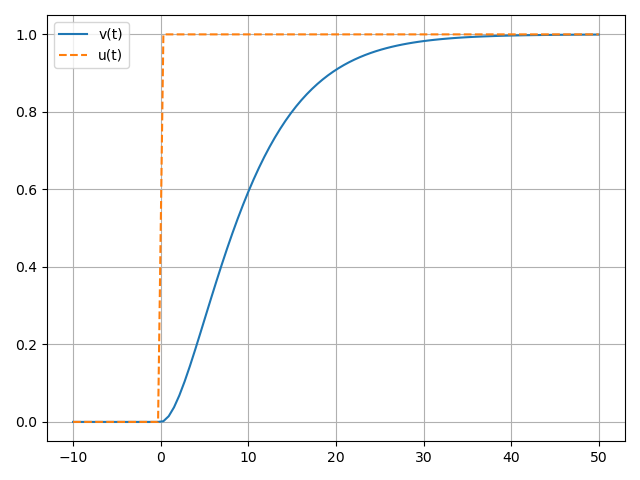
\includegraphics[scale=0.66]{../figures/second_degree_critical.png}
\end{center}
\end{minipage}

Questa rappresenta, in particolare, il caso ideale in cui l'uscita segue il segnale in entrata il più velocemente possibile.
Sistemi dinamici di secondo grado come le sospensioni delle automobili vengono solitamente tarati per essere il più vicini allo smorzamento critico possibile (nel caso particolare delle automobili, si tende ad un leggero sottosmorzamento per aumentare il comfort).

\subsubsection{$\mathbf \Delta < 0$, poli complessi coniugati}
Vediamo infine il caso con poli complessi coniugati.
Avremo quindi che questi rispettano la forma:
$$
p_{1,2} =  - \left( \alpha \pm i \beta \right)
$$
con:
$$
\alpha = -\frac{a_1}{2a_2}, \quad \beta = \sqrt{ \frac{a_0}{a_2} - \left( \frac{a_1}{2 a_2} \right)^2 } = \sqrt{ \frac{a_0}{a_2} \left( 1 - \frac{a_1^2}{4 a_2 a_0} \right) }
$$
che derivano direttamente da $p_1$ e $p_2$ come li avevamo definiti con la formula quadratica (portando $2 a_2$ dentro per $\beta$, che è il termine radicale col radicando cambiato di segno).

Possiamo ricavare due valori fisicamente significativi, che sono la \textbf{pulsazione di risonanza}:
$$
\omega = \sqrt{\frac{a_0}{a_2}}
$$
e lo \textbf{smorzamento}:
$$
\xi = \frac{a_1}{2 \sqrt{a_0 a_2}}
$$
sapendo che questa situazione darà solitamente comportamenti oscillatori smorzati o meno (non smorzati se $a_1 = 0$).

In particolare, la pulsazione di risonanza rappresenta la pulsazione che si avrebbe senza smorzamento, mentre la pulsazione effettiva sarà più piccola a seconda dello smorzamento effettivo. 

Varrà infatti, rispetto ai poli:
\[
	\begin{cases}
		\alpha = -\xi \omega = - \frac{a_1}{2 \sqrt{a_0 a_2}} \sqrt{ \frac{a_0}{a_2} } = -\frac{a_1}{2 a_2} \\
		\beta = \omega \sqrt{1 - \xi^2} = \sqrt{ \frac{a_0}{a_2} } \sqrt{ 1 - \frac{a_1^2}{4 a_0 a_2} } = \sqrt{ \frac{a_0}{a_2} \left( 1 - \frac{a_1^2}{4 a_0 a_2} \right) }
	\end{cases}
\]

Potremo quindi adottare le forme standard:
\begin{itemize}
	\item \textbf{Forma di Bode:} questa sarà:
$$
G(s) = G(0) \cdot \frac{ 1 }{ \frac{1}{\omega^2} \cdot s^2 + 2 \frac{\xi}{\omega} \cdot s + 1 }
$$
notando che:
\[
	\begin{cases}
		2 \frac{\xi}{\omega} = 2 \frac{a_1}{2 \sqrt{a_0 a_2}} \cdot \sqrt{\frac{a_2}{a_0}} = \frac{a_1}{a_0} \\
		\frac{1}{\omega^2} = \frac{a_2}{a_0}
	\end{cases}
\]
e quindi:
$$
G(s) = \frac{ G(0) }{ \frac{1}{\omega^2} \cdot s^2 + 2 \frac{\xi}{\omega} \cdot s + 1 } = \frac{ \frac{b_0}{a_0} }{ 1 + \frac{a_1}{a_0} s + \frac{a_2}{a_0} s^2} = \frac{b_0}{a_0 + a_1 s + a_2 s^2}
$$
cioè equivale alla forma standard.
	\item \textbf{Forma di Evans:} questa sarà:
$$
G(s) = \frac{ \frac{b_0}{a_2} }{ s^2 + 2 \xi \omega \cdot s + \omega^2 }
$$
cioè la stessa di sopra moltiplicata sopra e sotto per $\omega^2$.
\end{itemize}

Vediamo quindi la \textbf{risposta al gradino}.
Per fare ciò, notiamo che la trasformata di Laplace risulterà:
$$
Y(s) = G(s) \cdot U(s) = \frac{\frac{b_0}{a_2}}{s (s + p_1) (s + p_2)}
$$
con il solito $p_{1, 2} = -(\alpha \pm i \beta)$.
Si avrà quindi la forma:
$$
= \frac{A}{s} + \frac{B}{s + p_1} + \frac{B^*}{s + p_2}
$$
Con residui coniugati $B$ e $B^*$.
Il calcolo di $A$ è piuttosto facile:
$$
A = \lim_{s \rightarrow 0} \frac{ \frac{b_0}{a_2} }{ (s + p_1) (s + p_2) } = \frac{ \frac{b_0}{a_2} }{p_1 p_2} = \frac{b_0}{a_2} \cdot \frac{a_2}{a_0} = \frac{b_0}{a_0} = G(0)
$$
visto che:
$$
p_1 p_2 = \alpha^2 + \beta^2 = \frac{a_1^2}{4 a_2^2} + \frac{a_0}{a_2} \left( 1 - \frac{a_1^2}{4 a_0 a_2} \right) = \frac{a_0}{a_2}
$$

Lo stesso non si può dire per $B$ o $B^*$.
Decidiamo allora di impostare direttamente la forma $y(t)$:
$$
y(t) = \frac{b_0}{a_0} \left( 1 + A e^{\alpha t} \cos{\omega t} + B e^{\alpha t} \sin{\omega t} \right)
$$
che sarà in ogni caso combinazione lineare delle soluzioni che potremmo trovare dall'antitrasformata $\mathcal{L}^{-1} \left\{ Y(s) \right\}$.
Imponiamo quindi le condizioni iniziali $y(0) = 0$ e $y'(0) = 0$:
\[
	\begin{cases}
		y(0) =  \frac{b_0}{a_0} \left( 1 + A e^{\alpha t} \cos{\beta t} + B e^{\alpha t} \sin{\beta t} \right)
		= \frac{b_0}{a_0} \left( 1 + A \right) \\
		y'(0) = \frac{b_0}{a_0} \left( \alpha B \cos(\beta t) - \beta B e^{\alpha t} \sin(\beta t) + C \alpha e^{\alpha t}\sin(\beta t) + \beta C e^{\alpha t} \cos(\beta t) \right)
		= \frac{b_0}{a_0} \left( -\alpha + \beta C \right)
	\end{cases}
\]
$$
	\implies A = -1, \quad C = \frac{\alpha}{\beta}
$$
da cui l'equazione finale:
$$
y\left(t\right)=\frac{b_{0}}{a_{0}}\left(1-e^{\alpha t}\cos\left(\beta t\right)+\frac{\alpha}{\beta}e^{\alpha t}\sin\left(\beta t\right)\right)
$$

\noindent
\begin{minipage}{\textwidth}
vediamo il grafico di una classica funzione $y(t)$ di questo tipo, che viene detta anche \textbf{sottosmorzata}:
\begin{center}
	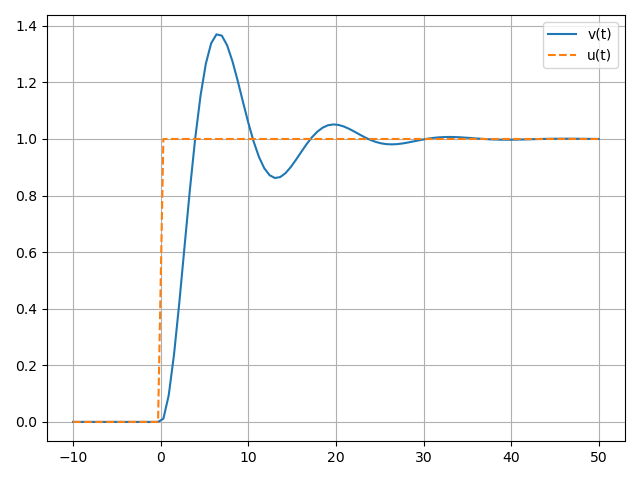
\includegraphics[scale=0.66]{../figures/second_degree_underdamped.png}
\end{center}
\end{minipage}

\subsubsection{Esempio: modello a quarto di automobile}
Prendiamo come esempio di sistema del secondo ordine quello del \textbf{quarto di automobile}.

Il sistema va inteso inteso come formato dalla massa dell'automobile $M_s$, che agisce sulla sospensione (di costante elastica $k_s$) e sull'ammortizzatore (di smorzamento $c$), a loro volta collegati alla ruota di massa $M_n$, il cui pneumatico che agisce anch'esso da sospensione (di costante elastica $k_p$) per il collegamento alla strada.
Prendiamo $x_s$ come la posizione verticale dell'auto, $x_n$ come la posizione verticale della ruota, e $x_f$ come la posizione verticale della strada (che \textit{varia} mentre la vettura si muove sul tracciato stradale, in base alle asperità stesse dell'asfalto).

Possiamo riportare la costante elastica del pneumatico (di per sé complicata da calcolare, e comunque solitamente abbastanza grande da essere considerata come perfettamente solida) alla sospensione, considerando quindi la sola costante elastica $k_s$ della sospensione.

\noindent
\begin{minipage}{\textwidth}
I grafici della situazione descritta, e della semplificazione che facciamo rimuovendo l'elasticità di pneumatico, saranno i seguenti: 

\begin{figure}[H]
    \centering
    \begin{subfigure}{0.45\textwidth}
        \centering
        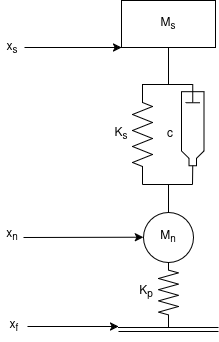
\includegraphics[scale=0.6]{../figures/suspension_complex.png}
        \caption{Quarto di automobile completo}
        \label{fig:image1}
    \end{subfigure}
    \hfill
    \begin{subfigure}{0.45\textwidth}
        \centering
        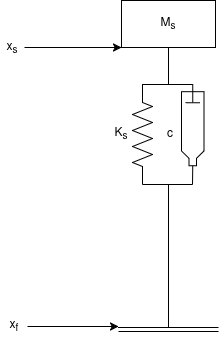
\includegraphics[scale=0.6]{../figures/suspension_simple.png}
        \caption{Quarto di automobile semplice}
        \label{fig:image2}
    \end{subfigure}
\end{figure}
\end{minipage}

\par\medskip

Prendiamo quindi la posizione verticale dell'automobile $x_s$ come l'uscita del sistema, e la posizione verticale della strada $x_f$ come l'entrata.

Chiamando poi $L_r$ la lunghezza della molla a riposo, potremmo impostare l'equazione differenziale come:
$$
M_s \frac{d^2 x_s}{dt^2} = c \frac{d ( x_f - x_s )}{dt} + k_s (x_f - x_s) + k_s L_r - M_s g
$$
dove il termine $k_s L_r$ deriva effettivamente dal fatto che la molla della sospensione risponde alla variazione della lunghezza a riposo della molla:
$$
F_s \propto  L_r - (x_s - x_f) = x_f - x_s + L_r
$$
mentre tutti i termini derivati non risentono di questa $L_r$ e quindi chiaramente la ignorano.

Dividiamo quindi la differenziale in una soluzione particolare, o di equilibrio, $\overline{x}_s$, e in una soluzione generale $\Delta x_s$:
$$
x_s = \Delta x_s + \overline{x}_s
$$
La condizione di equilibrio di questo sistema sarà quindi, imponendo derivate nulle:
$$
\overline{x}_s = L_r - \frac{M_s g}{k_s}
$$

Potremo allora prendere l'omogenea per il calcolo della soluzione generale:
$$
M_s \frac{d^2 \Delta x_s}{dt^2} = c \frac{d ( x_f - \Delta x_s )}{dt} + k_s (x_f - \Delta x_s)
$$
Raggruppando ingressi e uscite (rispettivamente, $\Delta x_s$ e $x_f$) si ha:
$$
M_s \frac{d^2 \Delta x_s}{dt^2} + c \frac{d \Delta x_s}{dt} + k_s \Delta x_s = c \frac{dx_f}{dt} + k_s x_f
$$
da cui, portandosi, al dominio di Laplace:
$$
\left( s^2 M_s + cs + k_s \right) \Delta x_s = ( cs + k_s ) x_f
$$
troviamo la funzione di trasferimento $G(s)$:
$$
G(s) = \frac{\Delta x_s}{x_f} = \frac{c s + k_s}{s^2 M_s + c s + k_s}
$$

La funzione di trasferimento ha uno zero e due poli.
Possiamo quindi ricavarci pulsazione naturale ($\omega$) e smorzamento ($\xi$):
$$
\omega = \frac{k_s}{M_s}, \quad \xi = \frac{c}{2 \sqrt{k_s M_s}}
$$
da cui potremo ricavare la risposta come spiegato nelle ultime 3 sezioni.

In particolare, abbiamo detto che le sospensioni autombilistiche sono solitamente sottosmorzate, da cui potremo ricavare i termini di smorzamento e pulsazione effettivi come:
\[
	\begin{cases}
		\alpha = -\xi \omega\\
		\beta = \omega \sqrt{1 - \xi^2}
	\end{cases}
\]

A questo punto, definita una funzione $x_f(t)$ per l'altezza del fondo stradale, si potrà ricavare la posizione $x_s(t)$ dell'automobile come la convoluzione:
$$
\Delta x_s(t) = ( g(t) * x_f(t) )
$$
dove $g(t)$ rappresenta la risposta all'impulso del sistema, data da:
$$
g(t) = \mathcal{L}^{-1} \left\{ G(s) \cdot 1 \right\} = A e^{\alpha t} \cos(\beta t) + B e^{\alpha t} \sin(\beta t)
$$
cioè la forma che abbiamo trovato nella sezione 13.0.2, tolto il termine costante (visto che prendiamo la risposta all'impulso, un termine costante compare comunque in $\overline{x}_s$).
Vorremo quindi imporre a $g(t)$ le condizioni iniziali $y(0) = 0$ e $y'(0) = 1$, da cui:
$$
A = 0, \quad B = \frac{1}{\beta}
$$
da cui:
$$
g(t) = \frac{1}{\beta} e^{\alpha t} \sin(\beta t)
$$

\end{document}
